%% USPSC-Cap3-Conclusao.tex
% ---
% Conclusão
% ---
\chapter{Conclusion}
\label{ch:conclusion}

This work introduces a distributed reinforcement learning framework tailored for high-frequency trading environments,
based on a shared parallel environment architecture and an asynchronous messaging backbone.
The proposed system addresses several persistent limitations in traditional distributed RL approaches
including communication overhead, data staleness, and the computational inefficiency arising from duplicated environment simulations.
By reconfiguring the standard multi-agent interaction model into a parallelized,
shared-environment setting, this approach aimed to utilize compute resources more efficiently, while preserving---
if not enhancing---the statistical diversity of sampled trajectories.


\section{Results}
\label{sec:results}

Throughout the design and evaluation process, emphasis was placed on reducing the straggler problem extend improving training throughput.
The use of a brokerless ZeroMQ Router/Dealer communication layout enabled asynchronous, low-latency interactions between workers and the central learner.
This design reduced idle time in the learning loop and facilitated scalable coordination across heterogeneous agents operating at different speeds.

The experimental results substantiate several of the design hypotheses.
As shown in \cref{tab:benchmarks}, using a centralized policy for batched inference dramatically reduced the average time spent in the `act' step,
where the learner generates the action tensor to be sent to the environments.
When the state tensors are centralized and batched for the policy network forward pass, which we named \textit{centralized policy},
the wall time was just $3.113$ milliseconds per timestep, while forward passing the state space independently per worker, named \textit{distributed policy}
was much slower, at about $35.142$ milliseconds per timestep.

\begin{table}[h!]
    \centering
    \begin{tabular}{|c|c|c|c|}
        \hline
        \textbf{Operation} & \textbf{Distributed Policy} & \textbf{Centralized Policy} \\
        \hline

        Act                & \SI{35.142}{\milli\second}  & \SI{3.113}{\milli\second}   \\
        Step               & \SI{40.554}{\milli\second}  & \SI{47.984}{\milli\second}  \\
        Reset              & \SI{12.709}{\micro\second}  & \SI{12.302}{\micro\second}  \\
        \hline
    \end{tabular}
    \caption{Trainer time benchmarks for ten worker instances. All operations are the average time for 100 episodes taken for each operation per rollout.}
    \label{tab:benchmarks}
\end{table}

The main contribution of this work is the empirical demonstration that asynchronous environment dynamics
can be shared between multiple learners to reduce redundant computations, while retaining stability for non-stationary simulators representative of financial market dynamics.
These dynamics, characterized by frequent regime shifts and exogenous shocks, are particularly prone to introducing non-Markovian effects that degrade learning performance.
The architecture’s ability to tolerate these conditions and increase learning efficiency highlights its applicability to real-world algorithmic trading systems.
To test our hypothesis that the PEARL framework is able to efficiently reuse simulator dynamics, we conducted tests using two trainers with $n$ environments,
ranging from $1$ to $32$ increasing in powers of $2$, that is, $n \in \left\{1, 2, 4, 8, 16, 32\right\}$.
We then recorded the episodic loss for $k = 10$ iterations per number of environment, at the end of $100$ episodes, averaging them into a single loss curve per environment count.
In \cref{fig:loss}, we plot the episodic loss, and in \cref{fig:performance} we plot the final average negative log loss per count of shared environments.
The performance at the end of the $100$ episodes scales positively with the number of shared environments, up to $8$ environments,
when it starts to decrease.
We attribute this behavior to the test machine's $8$ physical CPU cores, which limit training scalability.
Increasing the number of environments beyond the available cores introduced enough context-switching overhead to outweigh additional performance gains.

\begin{figure}[htbp]
    \begin{minipage}[t]{0.48\textwidth}
        \centering
        \includegraphics[width=\textwidth]{images/results/loss_episode}
        \caption{Average training loss over time for the shared environment architecture.}
        \label{fig:loss}
    \end{minipage}
    \hfill
    \begin{minipage}[t]{0.48\textwidth}
        \centering
        \includegraphics[width=\textwidth]{images/results/performance}
        \caption{Performance comparison of the shared environment for different numbers of shared environments.}
        \label{fig:performance}
    \end{minipage}
\end{figure}

While the system achieves positive results when increasing shared environments, both in terms of latency and compute utilization,
it also poses a discussion on the trade-offs of shared LOB environments.
The increased number of environments proportionally increases contention on the simulation process, which becomes a bottleneck under extremely high agent concurrency.
This can be seen in \cref{fig:speedup}, which shows the speedup for the different counts of shared environments.
As the number of environments increases, the processing speed, that is, how fast the concurrent environments can sample and insert new orders into the LOB,
decreases exponentially.
Additionally, managing consistent rollout recording and replay in this context requires careful attention to buffering and message timing.
These aspects open future directions for improvement, such as adaptive load balancing across simulation shards, environment step batching,
and most promisingly is accelerating environment processing speeds using model-based simulations.

\begin{figure}
    \centering
    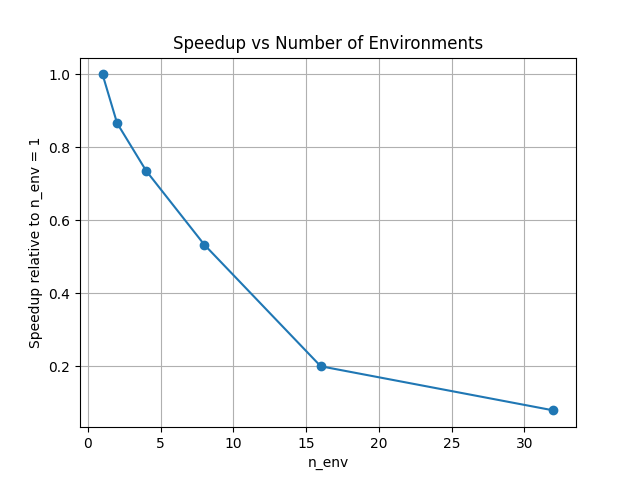
\includegraphics[width=0.6\textwidth]{images/results/speedup}
    \caption{Performance comparison of the shared environment for different numbers of shared environments.}
    \label{fig:speedup}
\end{figure}

\begin{table}[h!]
    \centering
    \renewcommand{\arraystretch}{1.2}
    \begin{tabularx}{\textwidth}{|c|X|X|}
        \hline
        \textbf{n} & \textbf{Episodic training loss} & \textbf{Total wall time (s)} \\
        \hline
        1          & 0.702 ± 0.694                 & 37.57 ± 0.40             \\
        2          & 0.855 ± 0.157                 & 43.37 ± 0.74             \\
        4          & 0.559 ± 0.087                 & 51.07 ± 0.21             \\
        8          & 0.382 ± 0.088                 & 70.48 ± 0.40             \\
        16         & 0.532 ± 0.183                 & 187.92 ± 1.10            \\
        32         & 0.525 ± 0.124                 & 475.85 ± 44.39           \\
        \hline
    \end{tabularx}
    \caption{
        Summary of loss and wall time (mean ± std) for training $2$ learners, averaged over 10 iterations prematurely ended at 100 episodes.
        $\textbf{n}$ is the number of shared environments running in parallel.
    }
    \label{tab:summary}
\end{table}


\section{Discussion}
\label{sec:discussion}

The tests performed in the previous section allowed us to evaluate the performance and scalability of the proposed RL framework in the context of high-frequency trading.
The obtained results corroborated that reducing the number of replicated simulator dynamics for individual workers could be avoided
by sharing environment dynamics across multiple learners, which in turn increased the overall training performance.

An additional result was the use of a centralized policy in the training process which also dramatically helped reduced per-timestep latency.

In summary, this work contributed with:
\begin{itemize}
    \item An asynchronous architecture based on shared environments for distributed RL;
    \item A high-throughput, low-latency communication layer based on a brokerless messaging queue;
    \item Empirical evidence of improved performance by means of lower training losses for similar training times under realistic simulators;
    \item Performance evaluation of a multi-agent, multi-environment market making policy under non-stationary, non-Markovian conditions.
\end{itemize}

Additionally, the modular nature of the proposed PEARL architecture supports heterogeneous learners by allowing each instance to use a different algorithm
for each learner instance, so traders can test and train multiple different strategies together and independently.
Although fully developed, the architecture does not allow for strategies to communicate between each other,
and thus could be further extended to support Multi-policy learning (e.g., mixture-of-experts models).
Another promising topic for future research that could improve the overall performance of the system is adaptive population scheduling
—dynamically allocating computational resources to learners based on their performance.
Adaptative population scheduling could reduce strategy exploration and exploitation costs greatly,
and enable fund managers to adaptively prioritize profitable strategies, especially in capital-constrained environments.

The results presented here demonstrate the feasibility and potential of designing systems that balance the algorithmic sophistication of
modern RL methods with the practical constraints and nature of high-frequency trading infrastructure.
The proposed framework provides a practical and scalable foundation for building high-performance simulators,
suitable for both academic research and real-time deployment in autonomous trading systems.
